\documentclass[12pt]{article}

\usepackage{url}
\usepackage{fullpage}
\usepackage{amssymb,amsfonts}
\usepackage{amsmath}
\newcommand{\eps}{\varepsilon}
\newcommand{\R}{\mathbb{R}}

\usepackage{listings}
\usepackage{color}
\usepackage{graphicx}

\usepackage{varwidth}

\usepackage{longtable}

\usepackage{hyperref}
\hypersetup{
    linktoc=all,     %set to all if you want both sections and subsections linked
    colorlinks=true,
    linkcolor=blue,
    filecolor=magenta,      
    urlcolor=cyan,
}

\definecolor{dkgreen}{rgb}{0,0.6,0}
\definecolor{gray}{rgb}{0.5,0.5,0.5}
\definecolor{mauve}{rgb}{0.58,0,0.82}

\lstset{frame=tb,
  language=Python,
  aboveskip=3mm,
  belowskip=3mm,
  showstringspaces=false,
  columns=flexible,
  basicstyle={\small\ttfamily},
  numbers=none,
  numberstyle=\tiny\color{gray},
  keywordstyle=\color{blue},
  commentstyle=\color{dkgreen},
  stringstyle=\color{mauve},
  breaklines=true,
  breakatwhitespace=true,
  tabsize=3
}

\usepackage[toc,page]{appendix}

\DeclareMathOperator*{\E}{\mathbb{E}}
\let\Pr\relax
\DeclareMathOperator*{\Pr}{\mathbb{P}}

\DeclareMathOperator*{\Lap}{\text{Lap}}

\DeclareMathOperator*{\Geo}{\text{Geo}}

\def\cl{\lstinline}

\title{CS 208 Homework 4a}
\author{Andrew Shackelford}
\date{April 16, 2019}
\setcounter{tocdepth}{3}

\begin{document}

\maketitle

\textbf{All code and figures are available \href{https://github.com/andrew-shackelford/cs208/tree/master/4a}{here}}.

{
  \hypersetup{linkcolor=black, hidelinks}
  \tableofcontents
}

\newpage

\section{Problem 1}

\subsection{Part A}

\subsubsection{Centralized Model}

\noindent

To implement the centralized model, we will add Laplace noise to each $p_j$ estimate. The global sensitivity of $p_j = \frac{1}{n}$, since each $x_i$ contribution to $p_j$ is either 0 or 1, and $p_j$ is a mean of $n$ of those contributions. Since we are dividing the privacy budget equally among each of the $d$ estimates, the scale of the noise is equal to $\frac{\text{sensitivity} \cdot d}{\epsilon} = \frac{d}{n \cdot \epsilon}$. The implementation of the centralized model is located in the \cl{centralized_mechanism} function of \cl{problem_1.py}, located at Appendix \ref{appendix:problem_1}.

\subsubsection{Local Model}

\noindent

For the local model, each data point $(x_i, y_i)$ does an randomized response on each $p_j$. Therefore, after each data point's individual $p_j$ is calculated, we return $p_j$ with probability $\frac{e^\epsilon}{e^\epsilon + 1}$, and $-p_j$ with probability $\frac{1}{e^\epsilon + 1}$ (after first scaling our $p_j$ from $\{0, 1\}$ to $\{-1, 1\}$). Then, when aggregating, we use the scale factor $c = \frac{e^\epsilon + 1}{e^\epsilon - 1}$ and then scale back from $[-1, 1]$ (+ noise) to $[0, 1]$ (+ noise). The implementation of the local model is located in the \cl{local_mechanism} function of \cl{problem_1.py}, located at Appendix \ref{appendix:problem_1}.

\subsection{Part B}

\subsubsection{Centralized Model}

\noindent

$\Pr[\hat{S} \not \supseteq S]$ is the probability that $\hat{S}$ does not have an element that is in $S$. For an element to be in $S$ that is not in $\hat{S}$, there must be at least one $p_j$ for an element $j \in S$ that is greater than our threshold $t$, thus causing it to not be included in $\hat{S}$. Since we are dealing with the ``realizable'' case of learning where the non-noisy $p_j = 0$, this means that the Laplace noise $\alpha$ we added must be greater than the threshold, in fact, strictly greater, not greater in absolute value, since our threshold will accept negative values of $p_j$ just fine. The probability that this noise $\alpha \leq t$ is equal to the Laplace CDF $F(t)$. $F(t) = 1 - \frac{1}{2} \exp(-\frac{t - \mu}{b})$, where $\mu$ is the mean and $b$ is the scale. Our $\mu = 0$, and $b$ is the scale we discussed in part 1.1.1, which is equal to $\frac{d}{n \cdot \epsilon}$. Therefore, $F(t) = 1 - \frac{1}{2} \exp(-\frac{t \cdot n \cdot \epsilon}{d}) = \Pr[\alpha \leq t]$, In order for $\hat{S} \not \supseteq S$, one of these probabilities must be unsatisfied for an element in $S$. Therefore, $\Pr[\hat{S} \not \supseteq S]$ is equal to 1 - the product of $d$ probabilities that each $p_j \leq t$. As a result, $\Pr[\hat{S} \not \supseteq S] = 1 - [1 - \frac{1}{2} \exp(-\frac{t \cdot n \cdot \epsilon}{d})]^{|S|} \leq 1 - [1 - \frac{1}{2} \exp(-\frac{t \cdot n \cdot \epsilon}{d})]^{d}$. Solving for $t$ to ensure $\Pr[\hat{S} \not \supseteq S] \leq 0.1$:

\begin{align*}
\Pr[\hat{S} \not \supseteq S] &\leq 0.1 \\
1 - [1 - \frac{1}{2} \exp(-\frac{t \cdot n \cdot \epsilon}{d})]^{d} &\leq 0.1 \\
0.9 &\leq [1 - \frac{1}{2} \exp(-\frac{t \cdot n \cdot \epsilon}{d})]^{d} \\
\sqrt[d]{0.9} &\leq 1 - \frac{1}{2} \exp(-\frac{t \cdot n \cdot \epsilon}{d}) \\
\frac{1}{2} \exp(-\frac{t \cdot n \cdot \epsilon}{d}) &\leq 1 - \sqrt[d]{0.9} \\
\exp(-\frac{t \cdot n \cdot \epsilon}{d}) &\leq 2 - 2\sqrt[d]{0.9} \\
-\frac{t \cdot n \cdot \epsilon}{d} &\leq \ln[2 - 2\sqrt[d]{0.9}] \\
\frac{t \cdot n \cdot \epsilon}{d} &\geq -\ln[2 - 2\sqrt[d]{0.9}] \\
t &\geq -\frac{d}{n \cdot \epsilon} \ln[2 - 2\sqrt[d]{0.9}] \\
\end{align*}


\subsubsection{Local Model}

\bigskip

\noindent

Like above, the probability that $\hat{S}$ does not have an element that is in $S$ is 1 - the product of $d$ probabilities that each $p_j$ is less than the threshold $t$. However, the $p_j$'s are calculated differently. Each $p_j$ is the mean of $n$ randomized responses. Note that we will not use a scaling factor since we aim not to estimate the population mean, but will instead use a binomial variable to be described below. The individual $p_j$'s from each user, which we will designate $p_{ji}$, have probability $\frac{e^{\epsilon/d}}{1 + e^{\epsilon/d}}$ of being the true response, and probability $\frac{1}{1 + e^{\epsilon/d}}$ of being the false response, since we have to divide our privacy budget $\epsilon$ over $d$ responses. For any element $j \in S$, we know the true $p_j = 0$ since this is the realizable case of learning. Therefore, we can view the false response as a ``1'', and the true response as a ``0'', since each false response will contribute to $p_j$ while each true response will not.

\medskip

We can view this as a binomial distribution, and approximate the sum of the binomial distributions $\mathcal{B}(\frac{1}{1 + e^{\epsilon/d}}, \frac{e^{\epsilon/d}}{1 + e^{\epsilon/d}})$ over $n$ samples with a normal distribution $\mathcal{N}(n\frac{1}{1 + e^{\epsilon/d}}, n\frac{e^{\epsilon/d}}{1 + e^{\epsilon/d}}\frac{1}{1 + e^{\epsilon/d}}) = \mathcal{N}(\frac{n}{1 + e^{\epsilon/d}}, \frac{n \cdot e^{\epsilon/d}}{(1 + e^{\epsilon/d})^2})$. Since we aim to take the mean of the $p_j$'s, we will multiply this by $\frac{1}{n}$. Thus, the normal distribution is given by $\mathcal{N}(\frac{1}{1 + e^{\epsilon/d}}, \frac{e^{\epsilon/d}}{n \cdot (1 + e^{\epsilon/d})^2})$. Now, we must find the probability that this normal distribution is less than the threshold $t$. Using the CDF of the normal distribution, the probability that one $p_j \leq t$ is equal to $F(t)$, where $F$ is the CDF of the normal distribution given by $\mathcal{N}(\frac{1}{1 + e^{\epsilon/d}}, \frac{e^{\epsilon/d}}{n \cdot (1 + e^{\epsilon/d})^2})$.  As a result, the probability that at least one of the $p_j > t$ is equal to $1 - F(t)^{|S|} \leq 1 - F(t)^d$. Solving for $t$:

\begin{align*}
\Pr[\hat{S} \not \supseteq S] &\leq 0.1 \\
1 - F(t)^d &\leq 0.1 \\
0.9 &\leq F(t)^d \\
\sqrt[d]{0.9} &\leq F(t) \\
F^{-1}(\sqrt[d]{0.9}) &\leq t \\
\end{align*}

where $F(t)$ is the Normal CDF with mean $\frac{1}{1 + e^{\epsilon/d}}$ and variance $\frac{e^{\epsilon/d}}{n \cdot (1 + e^{\epsilon/d})^2}$.

\subsection{Part C}

\subsubsection{Process}

\noindent

The code for this analysis is located in \cl{problem_1.py}, located at Appendix \ref{appendix:problem_1}. In order to train our classifier, we will use the thresholds described in Part B. If the $p_j$ for a given variable is less than the threshold, we will mark it as one of the predictors in our conjuction, otherwise we will exclude it. Since we aim to predict based on a conjuction of demographic characteristics, not the variables themselves, we first have to add each variable with its bits flipped to our dataset, so that we can predict with either characteristic, not just the value that is coded as 1.

\bigskip

The \cl{test_success} function contains code that does the following:
\begin{itemize}
  \item For no privacy, centralized DP, and local DP:
  \begin{itemize}
    \item Calculate the $p_j$'s
    \item Determine what $x$ variables the classifier would predict given the $p_j$'s
    \item Calculate the false positive and negative rates given the classifier's predictions
  \end{itemize}
\end{itemize}

\bigskip

The \cl{false_rates} function contains code that does the following:
\begin{itemize}
  \item For each bootstrap size in a range of $[10^{-5} \cdot n, n]$:
  \begin{itemize}
    \item For 100 trials:
    \begin{itemize}
      \item Create a bootstrapped dataset of that size
      \item Calculate the centralized and local DP results for the bootstrapped dataset
      \item Determine the false positive and negative rates for each set of results
    \end{itemize}
  \end{itemize}
\end{itemize}

\subsubsection{Results}

\noindent

Our classifier with no privacy determined that variables (indexed from 0) [5, 7, 9, 10] would correctly predict the targetted variable, which correspond to ``employed'', ``uscitizen'', ``englishability'', and the inverse of ``sex'' (that is, male instead of female). Therefore, we determined that the interest group is targeting employed male US citizens who speak English.

\bigskip

Our centralized DP classifier also predicted the correct variables, while our local DP classifier did not. Since the epsilon was so small ($\frac{1}{20} = 0.05$, which correlates to a true response probability of $51.2\%$), it was very difficult for the local DP classifier to separate out which variables had lower $p_j$'s due to noise. While the local DP classifier would include different combinations of extra variables (typically some subset of [12, 13, 18]) each time, it rarely if ever correctly predicted exactly [5, 7, 9, 10].

\bigskip

This analysis continued in our calculations of false positive and false negative rates. Below are two plots of the false positive and false negative rates for both the local and centralized mechanisms:

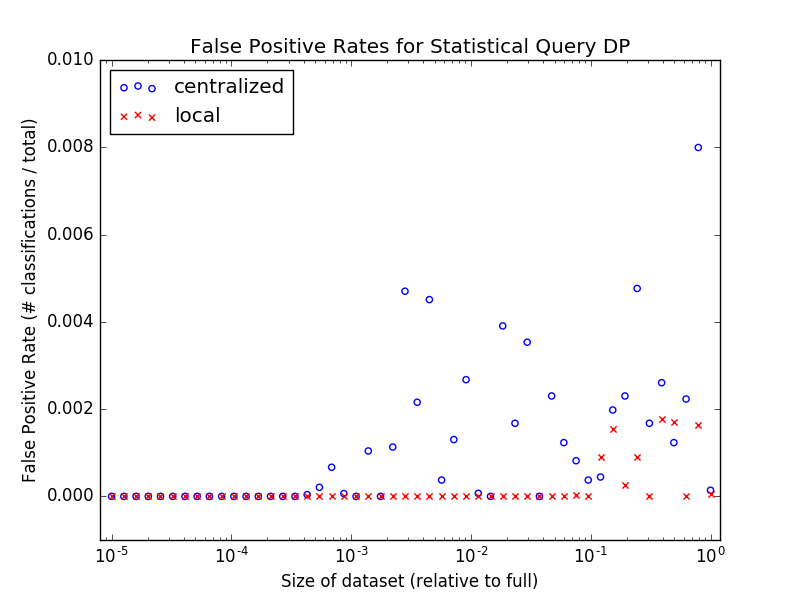
\includegraphics[scale=0.5]{false_positive_rate.png}

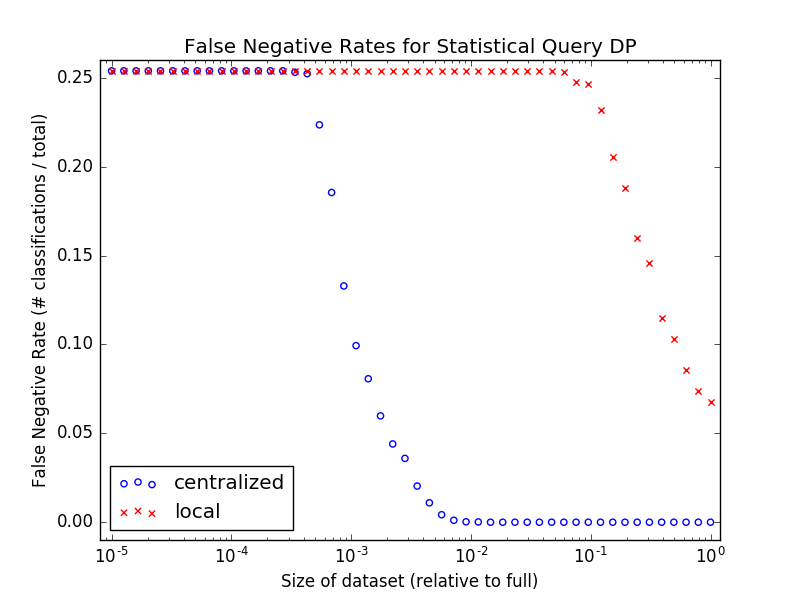
\includegraphics[scale=0.5]{false_negative_rate.png}

\subsubsection{Analysis}

\noindent

Looking at the results, we observe two main things. First, the false positive rates are comfortably within our bounds. We never achieve a false positive rate above 0.008. While there is no direct correlation between $\Pr[\hat{S} \not \supseteq S]$ and our false positive classification rate, we can clearly observe that at the very least our threshold calculation seems to be working. Secondly, we see that the centralized DP mechanism starts working (that is, the false negative rates approach 0) sooner than the local DP mechanism. This makes intuitive sense, as we know that centralized DP requires less noise, and thus would start working on a smaller dataset than local DP.

\bigskip

This still begs the question, however, of when local DP would start to work. Experimentally, even with a bootstrapped dataset of size $10n$, the local DP mechanism still failed repeatedly. I attempted to run the local DP mechanism on a synthetic dataset of size $100n$, however that required over 25 GB of RAM (on a laptop that has 8 GB) and caused my computer to become inoperable. During testing, I ran the local DP mechanism on the dataset without the additional flipped variables, and it was successful at predicting the variables correctly (at least on the variables present). Since adding the flipped variables cut our $\epsilon$ by an additional factor of 2, it seems likely that the local DP algorithm would eventually work on a sufficiently large dataset. However, experimentally confirming this is infeasible on a 2015-era laptop. This highlights the inherent problems with local DP -- large datasets are required, and performing the analysis can be costly, especially with low values of $\epsilon$.


\newpage

\begin{appendices}

\section{\cl{problem_1.py}}
\label{appendix:problem_1}

\begin{lstlisting}
"""
Andrew Shackelford
ashackelford@college.harvard.edu

CS 208 - Spring 2019
Homework 4a, Problem 1
"""

import numpy as np
import matplotlib.pyplot as plt
import csv
from scipy.stats import norm
import pickle

false_rates_dict = {}

# read in the data from the CSV file
def read_data(file):
    with open(file, 'rb') as f:
        next(f) # skip labels
        X, Y = [], []
        reader = csv.reader(f)
        for row in reader:
            res_x = []
            x = map(int, row[:-2]) # map input to integers
            flip_x = map(lambda n: 1 ^ n, x) # flip bits
            res_x.extend(x)
            res_x.extend(flip_x)

            X.append(res_x)
            Y.append(int(row[-1]))

        return np.array(X), np.array(Y)

# generate true probabilities
def true_data(X, Y):
    p = np.zeros(X.shape)
    for j in range(X.shape[1]):
        X_j = X[:, j]
        for i in range(X.shape[0]):
            p[i][j] = int(X_j[i] == 0 and Y[i] == 1)
    return p

# return mean for true probabilities
def true_mechanism(p):
    p_mean = np.zeros(p.shape[1])
    for j in range(p.shape[1]):
        p_j = p[:, j]
        p_mean[j] = np.mean(p_j)
    return p_mean

# return centralized dp mean
def centralized_mechanism(p, epsilon):
    p_mean = true_mechanism(p)
    p_dp = np.zeros(p_mean.shape)

    sensitivity = 1. / float(p.shape[0])
    scale = float(p.shape[1]) * sensitivity / float(epsilon)
    for j in range(p.shape[1]):
        p_dp[j] = p_mean[j] + np.random.laplace(scale=scale)

    return p_dp

# return localized dp mean using randomized response
# if desired, use scale_result to try to estimate the population mean
# however, this is not needed with our threshold from our normal approx.
def local_mechanism(p, epsilon, scale_result=False):
    # divide epsilon by d
    epsilon = float(epsilon) / float(p.shape[1])

    # calcuate probabilities and scaling factor
    true_prob = np.exp(epsilon) / (np.exp(epsilon) + 1.)
    false_prob = 1. / (np.exp(epsilon) + 1.)
    c = (np.exp(epsilon) + 1.) / (np.exp(epsilon) - 1)
    probs = [true_prob, false_prob]

    # perform randomized response
    choices = np.random.choice([1, -1], size=p.shape[0]*p.shape[1], replace=True, p=probs)
    choices = choices.reshape(p.shape)
    p_dp = np.multiply(p, choices) # perform multiplication instead of if/else for runtime savings
    p_dp_mean = np.mean(p_dp, axis=0)

    # scale the results back to [0, 1] (+ noise), with scaling factor if desired
    p_res = np.zeros(p_dp_mean.shape)
    for j in range(p.shape[1]):
        if scale_result:
            p_res[j] = ((c * p_dp_mean[j]) + 1.) / 2.
        else:
            p_res[j] = (p_dp_mean[j] + 1.) / 2.

    return p_res

# calculate the threshold for centralized dp
def calculate_centralized_threshold(d, n, epsilon):
    d, n, epsilon = float(d), float(n), float(epsilon)

    ln_term = 2. - (2. * np.power(0.9, 1./d))
    coeff = -d / (n * epsilon)
    return coeff * np.log(ln_term)

# calculate the threshold for local dp
def calculate_local_threshold(d, n, epsilon):
    d, n, epsilon = float(d), float(n), float(epsilon) / float(d)

    inverse_cdf_term = np.power(0.9, 1./d)
    mu = 1. / (1. + np.exp(epsilon))
    variance = (np.exp(epsilon)) / (n * np.square(1. + np.exp(epsilon)))
    return norm.ppf(inverse_cdf_term, loc=mu, scale=np.sqrt(variance))

# given a threshold, return the x variables that pass
def threshold(p, t):
    return np.argwhere(p <= t).flatten()

# calculate the false pos and neg rates given the chosen indices
def calculate_false_rate(X, Y, indices):
    # use dictionary to avoid having to re-run expensive calculations
    global false_rates_dict
    if indices.tostring() in false_rates_dict:
        return false_rates_dict[indices.tostring()]

    num_false_pos, num_false_neg = 0, 0
    for i in range(X.shape[0]):
        if indices.shape[0] == 0:
            num_false_neg += 1
        else:
            predicted = np.min(X[i][indices])
            num_false_pos += max(0, predicted - Y[i])
            num_false_neg += max(0, Y[i] - predicted)

    false_rates_dict[indices.tostring()] = (num_false_pos, num_false_neg)
    return num_false_pos, num_false_neg

# print out x variables that pass as well as false pos and neg rates
# for true results, centralized dp, and local dp with given dataset
def test_success():
    # set constants, read in and scale data
    epsilon = 1.
    X, Y = read_data('CaPUMS5full.csv')
    p = true_data(X, Y)
    scaled_p = (p - 0.5) * 2

    # calculate true x variables, print out false positives and negatives for sanity check
    print "No Privacy:"
    result = threshold(true_mechanism(p), 0.00000001)
    print result
    print calculate_false_rate(X, Y, result)

    # perform centralized dp, print out results
    print "Centralized Mechanism:"
    t = calculate_centralized_threshold(p.shape[1], p.shape[0], epsilon)
    result = threshold(centralized_mechanism(p, epsilon), t)
    print result
    print calculate_false_rate(X, Y, result)

    # perform local dp, print out results
    print "Local Mechanism:"
    t = calculate_local_threshold(scaled_p.shape[1], scaled_p.shape[0], epsilon)
    result = threshold(local_mechanism(scaled_p, epsilon), t)
    print result
    print calculate_false_rate(X, Y, result)

# calculate centralized and local dp false rates over various bootstrapped datasets
def false_rates():
    # read in and scale data, calculate true result
    X, Y = read_data('CaPUMS5full.csv')
    p = true_data(X, Y)
    scaled_p = (p - 0.5) * 2
    true_result = threshold(true_mechanism(p), 0.00000001)

    # define constants, bootstrap sizes
    epsilon = 1.
    num_trials = 100
    bootstrap_sizes = np.logspace(-5, 0)
    centralized_false_pos_results, centralized_false_neg_results = [], []
    local_false_pos_results, local_false_neg_results = [], []

    for size in bootstrap_sizes:
        print size

        centralized_num_false_pos, centralized_num_false_neg = 0, 0
        for i in range(num_trials):
            # create bootstrap
            indices = np.random.choice(p.shape[0], size=int(size*p.shape[0]), replace=True)
            p_bootstrap = p[indices]
            scaled_p_bootstrap = scaled_p[indices]

            # perform dp analysis
            centralized_t = calculate_centralized_threshold(p_bootstrap.shape[1], p_bootstrap.shape[0], epsilon)
            centralized_result = threshold(centralized_mechanism(p_bootstrap, epsilon), centralized_t)
            local_t = calculate_local_threshold(p_bootstrap.shape[1], p_bootstrap.shape[0], epsilon)
            local_result = threshold(local_mechanism(p_bootstrap, epsilon), local_t)

            # calculate number of false pos and neg
            centralized_trial_pos, centralized_trial_neg = calculate_false_rate(X, Y, centralized_result)
            centralized_num_false_pos += centralized_trial_pos
            centralized_num_false_neg += centralized_trial_neg
            local_trial_pos, local_trial_neg = calculate_false_rate(X, Y, local_result)
            local_num_false_pos += local_trial_pos
            local_num_false_neg += local_trial_neg

        # calculate rates
        centralized_false_pos_rate = float(centralized_num_false_pos) / float(num_trials * p.shape[0])
        centralized_false_neg_rate = float(centralized_num_false_neg) / float(num_trials * p.shape[0])
        local_false_pos_rate = float(local_num_false_pos) / float(num_trials * scaled_p.shape[0])
        local_false_neg_rate = float(local_num_false_neg) / float(num_trials * scaled_p.shape[0])

        # append to results
        centralized_false_pos_results.append(centralized_false_pos_rate)
        centralized_false_neg_results.append(centralized_false_neg_rate)
        local_false_pos_results.append(local_false_pos_rate)
        local_false_neg_results.append(local_false_neg_rate)

    # write results to file
    with open('centralized_false_pos_results.pkl', 'wb') as f:
        pickle.dump(centralized_false_pos_results, f)
    with open('centralized_false_neg_results.pkl', 'wb') as f:
        pickle.dump(centralized_false_neg_results, f)
    with open('local_false_pos_results.pkl', 'wb') as f:
        pickle.dump(local_false_pos_results, f)
    with open('local_false_neg_results.pkl', 'wb') as f:
        pickle.dump(local_false_neg_results, f)

# graph the results
def graph_results():
    # load results from file
    with open('centralized_false_pos_results.pkl', 'rb') as f:
        centralized_false_pos_results = pickle.load(f)
    with open('centralized_false_neg_results.pkl', 'rb') as f:
        centralized_false_neg_results = pickle.load(f)
    with open('local_false_pos_results.pkl', 'rb') as f:
        local_false_pos_results = pickle.load(f)
    with open('local_false_neg_results.pkl', 'rb') as f:
        local_false_neg_results = pickle.load(f)

    # create x axis
    x = np.logspace(-5, 0)

    # plot false positive results
    plt.xscale('log')
    plt.scatter(x, centralized_false_pos_results, marker='o', edgecolors='blue', facecolors='none', label='centralized')
    plt.scatter(x, local_false_pos_results, marker='x', color='red', label='local')
    plt.xlim(8e-6, 1.2)
    plt.ylim(-0.001, 0.010)
    plt.legend(loc='upper left')
    plt.title('False Positive Rates for Statistical Query DP')
    plt.ylabel('False Positive Rate (# classifications / total)')
    plt.xlabel('Size of dataset (relative to full)')
    plt.savefig('false_positive_rate.png')

    # plot false negative results
    plt.clf()
    plt.xscale('log')
    plt.scatter(x, centralized_false_neg_results, marker='o', edgecolors='blue', facecolors='none', label='centralized')
    plt.scatter(x, local_false_neg_results, marker='x', color='red', label='local')
    plt.xlim(8e-6, 1.2)
    plt.ylim(-0.01, 0.26)
    plt.legend(loc='lower left')
    plt.title('False Negative Rates for Statistical Query DP')
    plt.ylabel('False Negative Rate (# classifications / total)')
    plt.xlabel('Size of dataset (relative to full)')
    plt.savefig('false_negative_rate.png')

def main():
    test_success()
    false_rates()
    graph_results()

if __name__ == "__main__":
    main()
\end{lstlisting}

\end{appendices}

\end{document}